\section{Active Perception Lifts Document Agents}
\label{sec:harness}

A frozen vision-language model and a code-capable reasoner can be wired into a DocVQA agent in many ways, and the wiring --- not the choice of either model --- is what moves accuracy. Holding both models fixed and varying only the scaffold spans roughly 25 ANLS points on the DocVQA-2026 validation set. We establish the challenge (the task resists both small and frontier-scale models), state the active-perception hypothesis, prove it under a controlled comparison, isolate the mechanism, and show it generalizes across model families.

\subsection{Evaluation setup}
\label{sec:setup}

The metric is binary ANLS at threshold 0.9, the official DocVQA-2026 scoring rule: a prediction earns credit only when its normalized Levenshtein similarity to the gold answer reaches 0.9, otherwise zero. All harness numbers below are reported as mean~$\pm$~std over $n{=}8$ independent trials on the DocVQA-2026 validation split (25 documents, 80 questions), micro-averaged per question, with a frozen Qwen3.5-27B (served with vLLM \citep{vllm}) as the VLM perception endpoint throughout. The reasoner's native thinking mode is disabled.

Disabling native thinking does not remove reasoning --- it \emph{relocates} it. These models emit their reasoning by default in a dedicated thinking channel; we turn that channel off, and because the harness parses only the fenced Python code, the model instead writes its reasoning as free text interleaved with its code actions. Reasoning is thus present every turn, inline rather than in a separate channel --- and the DSPy solvers \citep{dspy} make it explicit, declaring a reasoning field in each turn's signature. Empirically the two settings are on par: disabling native thinking costs no measurable accuracy, while native thinking was hang-prone at the 27B scale and slower. No-think is therefore the stable, efficient configuration, not an answer-without-reasoning handicap.

\subsection{The challenge: bare and frontier setups both fall short}

DocVQA-2026 documents are long, multi-page, high-resolution, and largely visual --- figures, plots, schematics, maps --- so the answer-bearing content is often non-textual and a single question usually requires locating the right page and region before reading it. The task resists both ends of the scale axis. In a bare setup, no-scaffold prompting and raw multi-image VLM calls score low: a single raw multi-image call reaches 20.47 ANLS, a single multimodal agent reading pages in its own context 22.34, and the official competition baseline 17.81. At the other end, frontier-scale frozen models only plateau --- the official ICDAR-2026 baselines place Gemini~3~Pro at 37.50 and Gemini~3~Flash at 33.75 on the same validation split, low for their size on documents this large. Scaling the model alone is not the answer.

\subsection{Harness design space and the active-perception hypothesis}

A document agent's design space spans a taxonomy of scaffolds, all sharing the same frozen Qwen3.5-27B VLM:

\begin{itemize}
\item \textbf{Raw multi-image VLM} --- one VLM call over all page images, no agent, using the \emph{same} minimal prompt as the active-perception scaffolds, so the only difference from a scaffold is the scaffold itself (the controlled no-scaffold baseline).
\item \textbf{Multimodal REPL agent} --- a single multimodal agent that pulls document pages into its own context with \texttt{display()} and reasons over them directly, with no VLM-tool call.
\item \textbf{Official baseline} --- the published DocVQA-2026 competition baseline: one VLM call with the kit's \emph{own} prompt (an external reference point). It is the same raw-VLM mechanism as the row above and differs only in the prompt.
\item \textbf{ReAct} --- a thought $\rightarrow$ tool $\rightarrow$ observation loop with the same VLM perception tools but \textbf{no Python REPL}. Its only perception actuators are whole-page VLM queries at fixed page granularity; it cannot crop, zoom, or do coordinate arithmetic.
\item \textbf{the REPL active-perception family} --- scaffolds whose action is Python executed in a persistent REPL, sharing a tool surface, prompt body, and the perception primitive \texttt{batch\_look}, an on-demand call to the frozen VLM perception tool against cropped or zoomed image regions. The family has two members. \textbf{RLM} (Recursive Language Models \citep{rlm}) holds state in a hidden interpreter namespace and compacts the rendered context across turns. \textbf{CodeAct} \citep{codeact} is its append-only twin --- identical tools and \texttt{batch\_look} perception call, but a strictly append-only chat transcript in which each turn extends the previous one and no earlier token is rewritten, the prefix-preserving property \S\ref{sec:scaffold} requires of a fine-tuning target. Neither reads OCR text; perception is purely visual.
\item \textbf{OCR-only control} --- the RLM scaffold with visual perception swapped for OCR text plus lexical search (OCR-only RLM), isolating the contribution of the visual modality.\footnote{OCR text is pre-extracted per page with Docling (figures and pictures described by a Granite-Vision model) and indexed for BM25 lexical search; the agent reads this text in place of querying the VLM.}
\end{itemize}

The hypothesis follows: what governs accuracy is the \textbf{REPL active-perception loop} --- code that issues on-demand visual queries (crop, zoom, coordinate arithmetic) against a frozen VLM and continues reasoning over what comes back --- not model scale and not a fixed-granularity tool loop. Figure~\ref{fig:arch} contrasts the active-perception scaffold with the REPL-less ReAct loop.

\begin{figure}[t]
\centering
\footnotesize
\resizebox{\columnwidth}{!}{%
\begin{tikzpicture}[
  font=\footnotesize,
  box/.style={draw,rounded corners,align=center,inner sep=2.5pt,minimum height=0.62cm,text width=2.3cm},
  lm/.style={box,draw=blue!55,fill=blue!7},
  repl/.style={box,draw=green!45!black,fill=green!8},
  vlm/.style={box,draw=orange!75!black,fill=orange!9},
  doc/.style={box,draw=gray!60,fill=gray!10},
  fl/.style={-{Latex[length=1.6mm]},thick},
  node distance=0.42cm
]
% ---------- Panel A: active perception ----------
\node[font=\bfseries] (ta) at (0,0.5) {Active perception};
\node[lm]   (alm)  at (0,0)      {Reasoner-LM};
\node[repl] (arepl) [below=of alm] {Python REPL};
\node[vlm]  (avlm) [below=of arepl] {frozen VLM};
\node[doc]  (adoc) [below=of avlm] {document pages};
\draw[fl,blue!55]   (alm) -- node[right,font=\scriptsize]{writes code} (arepl);
\draw[fl,green!45!black] (arepl) -- node[right,font=\scriptsize]{\texttt{batch\_look}} node[left,font=\scriptsize]{crop/zoom} (avlm);
\draw[fl,orange!75!black] (avlm) -- (adoc);
\draw[fl,orange!75!black,dashed] (avlm.west) .. controls +(-1.1,0) and +(-1.1,0) .. node[left,font=\scriptsize]{obs}(arepl.west);

% ---------- Panel B: ReAct ----------
\node[font=\bfseries] (tb) at (4.6,0.5) {ReAct (no REPL)};
\node[lm]   (blm)  at (4.6,0)      {Reasoner-LM};
\node[vlm]  (bvlm) [below=0.84cm of blm] {frozen VLM};
\node[doc]  (bdoc) [below=of bvlm] {document pages};
\draw[fl,blue!55]   (blm) -- node[right,font=\scriptsize]{tool call} (bvlm);
\draw[fl,orange!75!black] (bvlm) -- node[right,font=\scriptsize]{whole page} (bdoc);
\draw[fl,orange!75!black,dashed] (bvlm.west) .. controls +(-1.0,0) and +(-1.0,0) .. node[left,font=\scriptsize]{obs}(blm.west);
\node[font=\scriptsize,gray!50!black,text width=2.6cm,align=center,below=0.3cm of bdoc]
  {no crop/zoom: perception fixed at page granularity};
\end{tikzpicture}%
}
\caption{The active-perception scaffold (left) inserts a Python REPL between reasoner and VLM, so the reasoner programs its perception --- cropping and zooming to image regions via \texttt{batch\_look}. ReAct (right) calls the same frozen VLM but without a REPL, so its only actuator is a whole-page query at fixed granularity. The REPL is the sole structural difference, and it is what converts reasoning into targeted perception (\S\ref{sec:mechanism}).}
\label{fig:arch}
\end{figure}

\subsection{Result: active perception dominates}

Table~\ref{tab:harness} compares the distinct harness designs under the common protocol, alongside two external frontier anchors; we defer ablations within a single design to \S\ref{sec:mechanism}. The designs fall into two tiers separated by a gap several times the within-tier standard deviation.

\begin{table*}[t]
\centering
\small
\begin{tabular}{llp{6.6cm}c}
\toprule
Tier & Solver & Mechanism & ANLS ($n{=}8$) \\
\midrule
\multirow{2}{*}{\emph{active perception}}
 & RLM & REPL + VLM perception tool \texttt{batch\_look}, OCR-free & \textbf{39.38 $\pm$ 1.49} \\
 & CodeAct & append-only twin, same tools & \textbf{39.53 $\pm$ 2.83} \\
\midrule
\multirow{4}{*}{\shortstack[l]{\emph{no active}\\\emph{perception}}}
 & ReAct & VLM tool, no REPL & 25.16 $\pm$ 4.60 \\
 & Multimodal REPL agent & REPL, pages in own context, no VLM-tool call & 22.34 $\pm$ 2.79 \\
 & Raw multi-image VLM & single VLM call, prompt matched to scaffolds & 20.47 $\pm$ 1.63 \\
 & Official baseline & competition kit's own prompt, one VLM call & 17.81 $\pm$ 1.86 \\
\midrule
\multirow{2}{*}{\emph{external anchor}}
 & Gemini 3 Pro & --- & 37.50 (val) \\
 & Gemini 3 Flash & --- & 33.75 (val) \\
\bottomrule
\end{tabular}
\caption{Harness-design comparison on DocVQA-2026 val (80Q), $n{=}8$, frozen Qwen3.5-27B VLM, no-think. The two tiers are separated by a gap several times the within-tier standard deviation. CodeAct is the corrected append-only loop (final, $n{=}8$).}
\label{tab:harness}
\end{table*}

The active-perception designs (RLM, CodeAct) reach $\sim$39 ANLS; every design that drops the REPL or the perception tool falls to 18--25. RLM, the reference active-perception result, reaches 39.38 and the append-only CodeAct ties it at 39.53 (within trial-to-trial variance), so the win belongs to the active-perception \emph{family} rather than a single harness --- a tie \S\ref{sec:scaffold} builds on. The family also matches or exceeds the official ICDAR-2026 frontier baselines on the same validation split (Gemini~3~Pro 37.50, Gemini~3~Flash 33.75): the advantage is not scale, since an active-perception scaffold on a 27B VLM reaches the accuracy of proprietary models many times larger.

\subsection{Mechanism: which components matter}
\label{sec:mechanism}

The mechanism is isolated two ways: by comparing RLM against the harness designs in Table~\ref{tab:harness} that drop one of its components, and by ablating one lever at a time within the RLM solver itself (Table~\ref{tab:ablation}). We keep the two apart deliberately --- Table~\ref{tab:harness} contrasts different designs; Table~\ref{tab:ablation}'s ablations all act on RLM.

\textbf{The REPL and the VLM perception tool are each necessary.} Removing either collapses the score. Stripping the REPL but keeping the perception tool (ReAct) drops the score by 14.2 relative to RLM; stripping the perception tool but keeping the REPL --- the Multimodal REPL agent, which loads pages into its own context instead --- drops it by 17.0; the no-agent baselines that drop both (Raw multi-image VLM 20.47, Official baseline 17.81) sit lower still. Neither half alone suffices.

\textbf{Within RLM, cropping and the visual modality are necessary; extra channels are not.} Table~\ref{tab:ablation} ablates one lever of the RLM solver at a time. Two levers carry the result. Restricting \texttt{batch\_look} to whole-page reads (removing crop/zoom) costs $-2.5$ overall but hits the detail-dense categories hardest --- engineering drawings and science posters, where zoom matters most; and replacing visual perception with OCR text collapses accuracy by 25.5 points to 13.91. The other directions are null-to-harmful: adding OCR text atop vision ($-1.6$), adding a direct \texttt{display()} image channel ($-3.9$), and generalizing the perception call into an arbitrary-subtask delegation tool ($-0.16$) none helps --- the lean, perception-only \texttt{batch\_look} is already at the optimum, and the extra channels mostly add noise.

\begin{table}[t]
\centering
\footnotesize
{\setlength{\tabcolsep}{4pt}
\begin{tabular}{lccp{1.7cm}}
\toprule
RLM ablation & ANLS & $\Delta$ & what it changes \\
\midrule
RLM (reference) & 39.38 & --- & perception-only \texttt{batch\_look}, crop/zoom, OCR-free \\
+ multi-modal sub-agent & 39.22 & $-0.16$ & generalize perception to any subtask \\
+ OCR & 37.81 & $-1.56$ & add OCR text + lexical search atop vision \\
$-$ crop/zoom & 36.88 & $-2.51$ & whole-page reads only \\
+ display channel & 35.47 & $-3.91$ & add a direct \texttt{display()} image channel \\
OCR-only & 13.91 & $-25.47$ & replace vision with OCR text \\
\bottomrule
\end{tabular}}
\caption{Ablations of the RLM solver --- one lever changed at a time, vs RLM (39.38), $n{=}8$ (ANLS@0.9, $\pm$std omitted; all within 1.5--4.5).}
\label{tab:ablation}
\end{table}

Both necessary levers act through \textbf{visual density}, not document length. At matched perception (a shared VLM, so the difference is purely harness), the RLM$-$ReAct gap is largest on visually dense categories --- engineering drawings, business reports, maps, infographics --- and smallest on text-linear ones --- scientific papers and slides (Figure~\ref{fig:category}); with a strong VLM the advantage is flat to slightly negative on the longest documents, where a whole-page read suffices once the answer page is found. The OCR-only collapse is graded the same way: the OCR-only agent scores \textbf{0/10 in all eight trials} on engineering drawings and maps, where the page is non-textual, and is most survivable on text-dense slides and scientific papers. Vision does the work OCR cannot, exactly where the content is not text. (These per-category gaps are computed on cross-model matched-config runs; the canonical absolutes are the $n{=}8$ numbers in Tables~\ref{tab:harness}--\ref{tab:ablation}.)

\begin{figure}[t]
\centering
\resizebox{\columnwidth}{!}{%
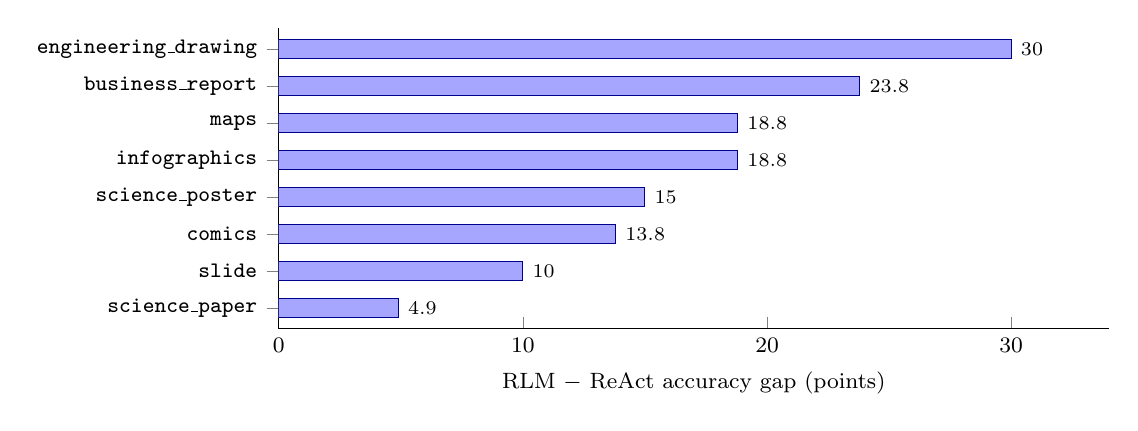
\begin{tikzpicture}
\begin{axis}[
  xbar, width=\columnwidth, height=5.4cm,
  bar width=7pt,
  enlarge y limits=0.08,
  xmin=0, xmax=34,
  xlabel={RLM $-$ ReAct accuracy gap (points)},
  xlabel style={font=\footnotesize},
  symbolic y coords={science\_paper,slide,comics,science\_poster,infographics,maps,business\_report,engineering\_drawing},
  ytick=data,
  yticklabel style={font=\footnotesize\ttfamily},
  xtick={0,10,20,30},
  tick label style={font=\footnotesize},
  nodes near coords, nodes near coords style={font=\scriptsize},
  nodes near coords align={horizontal},
  every node near coord/.append style={/pgf/number format/fixed,/pgf/number format/precision=1},
  axis x line*=bottom, axis y line*=left,
]
\addplot[draw=blue!55!black,fill=blue!35] coordinates {
  (4.9,science\_paper) (10.0,slide) (13.8,comics) (15.0,science\_poster)
  (18.8,infographics) (18.8,maps) (23.8,business\_report) (30.0,engineering\_drawing)
};
\end{axis}
\end{tikzpicture}%
}
\caption{The active-perception advantage tracks \textbf{visual density}. At matched perception (a shared 27B VLM, so the difference is purely harness), the RLM$-$ReAct accuracy gap by category is largest on detail-dense pages where cropping recovers fine structure (engineering drawings, business-report figures, maps, infographics) and smallest on text-linear ones (slides, scientific papers). Per-category cells are noisy (10 questions each); the ranking, not the exact value, is the point.}
\label{fig:category}
\end{figure}

\textbf{The REPL converts reasoning into perception.} A factorial swap separates the harnesses by what they are bound on. Replacing a weak reasoner on the 27B VLM with a strong 27B reasoner on a weaker 9B VLM \emph{gains} $+10.3$ for RLM and $+6.2$ for CodeAct (both reasoning-bound) but \emph{loses} $-3.05$ for ReAct (perception-bound). The REPL members write Python around \texttt{batch\_look} --- cropping to the evidence region, zooming, chaining successive crops, doing coordinate arithmetic --- so a stronger reasoner produces better-targeted perception queries and extracts more even from a weaker VLM. ReAct has no such actuator: its perception ceiling is the VLM's whole-page acuity, which a stronger reasoner cannot direct. The complementary swap confirms a perception bottleneck for mid and small reasoners: holding the reasoner fixed and upgrading its homogeneous VLM to the 27B VLM lifts accuracy $+7.9$ at the 9B reasoner (Welch $t{=}3.54$, 95\% CI [$+3.4$, $+12.3$]) and $+8.6$ at the 4B reasoner ($t{=}4.96$, 95\% CI [$+5.2$, $+12.0$]). The crop/zoom loop is the mechanism that turns reasoning capability into perception quality; remove it and reasoning can no longer buy perception.

\textbf{Effort is not accuracy.} Iteration count correlates negatively with success: $\mathrm{corr}(\text{iterations}, \text{accuracy}) \approx -0.31$ over 200 doc-trials, with accuracy falling $62.8\% \rightarrow 43.2\% \rightarrow 31.6\%$ across the 0--8 / 8--14 / 14+ iteration bins. The active-perception harnesses spend roughly twice the iterations and wall time of ReAct, but extra turns mark a hard document, not a path to the answer; the lever is the quality of the perception loop, not its length.

\textbf{A trajectory.} Figure~\ref{fig:trajectory} shows the loop on a single question over a 181-page document, trimmed verbatim from one agent trajectory. The agent surveys the document programmatically, locates the target table through a table-of-contents pointer, \emph{distrusts} the full-page VLM read and re-reads a tighter crop --- which disagrees, exposing a VLM misread --- adjudicates by reading the region in halves, and finally does the arithmetic the VLM cannot do, in Python. Every component of the mechanism appears in one trace, and the self-distrusting crop-verify is consequential rather than ceremonial: it catches a wrong number the whole-page read returned.

\begin{figure*}[t]
\centering
\footnotesize
\resizebox{\textwidth}{!}{%
\begin{tikzpicture}[
  font=\footnotesize,
  lm/.style={draw=blue!55,fill=blue!6,rounded corners,align=left,
             text width=4.3cm,inner sep=3pt,minimum height=0.8cm},
  vlm/.style={draw=orange!75!black,fill=orange!8,rounded corners,align=left,
              text width=3.6cm,inner sep=3pt,minimum height=0.8cm},
  call/.style={-{Latex[length=2mm]},blue!55,thick},
  ret/.style={-{Latex[length=1.6mm]},orange!75!black,thin,dashed,opacity=0.7}
]
% lane headers
\node[font=\small\bfseries,blue!55!black] at (2.2,0.75) {Reasoner-LM \;(writes Python)};
\node[font=\small\bfseries,orange!70!black] at (7.4,0.75) {frozen VLM \;(\texttt{batch\_look})};

% reasoner-LM lane (left)
\node[lm]  (s1) at (2.2,0)    {\textbf{1. Survey} 10 candidate pages in one batched call};
\node[lm]  (s2) at (2.2,-1.2) {\textbf{2. Locate} via a table-of-contents pointer};
\node[lm]  (s3) at (2.2,-2.4) {\textbf{3. Read} page 76 (full page)};
\node[lm,draw=red!60,fill=red!5]  (s4) at (2.2,-3.75)
     {\textbf{4. Distrust \& verify:} crop to the chart and re-read};
\node[lm]  (s5) at (2.2,-5.1) {\textbf{5. Adjudicate:} re-read top \& bottom halves separately};
\node[lm,fill=blue!12]  (s6) at (2.2,-6.55)
     {\textbf{6. Compute in Python} (arithmetic the VLM cannot do):\\
      \texttt{2287.07 $-$ 238.19} $\Rightarrow$ \textbf{SUBMIT 2048.88} \checkmark};

% VLM lane (right of divider)
\node[vlm] (r1) at (7.4,0)     {per-page summaries};
\node[vlm] (r2) at (7.4,-1.2)  {``the table is on p.\,76''};
\node[vlm] (r3) at (7.4,-2.4)  {\$2{,}287.07 \,/\, \$238.19};
\node[vlm,draw=red!60] (r4) at (7.4,-3.75)
     {\$978.42 \,/\, \$190.57\\\textbf{(disagrees!)}};
\node[vlm] (r5) at (7.4,-5.1)  {\$2{,}287.07 \,/\, \$238.19 \;\checkmark};

% request (LM->VLM) and return (VLM->next LM) arrows
\foreach \i in {1,2,3,4,5} {
  \draw[call] (s\i.east) -- (r\i.west);
  \draw[ret]  (r\i.south west) .. controls +(-0.5,-0.35) and +(0.5,0.35) .. (s\the\numexpr\i+1\relax.east);
}
% lane divider
\draw[gray!35,dashed] (4.9,1.0) -- (4.9,-7.2);
\draw[gray!35,dashed] (9.5,1.0) -- (9.5,-7.2);

% ---- document thumbnails (the active-perception crop) ----
\node[inner sep=0,draw=gray!55] (pagefull) at (14.9,0.05)
     {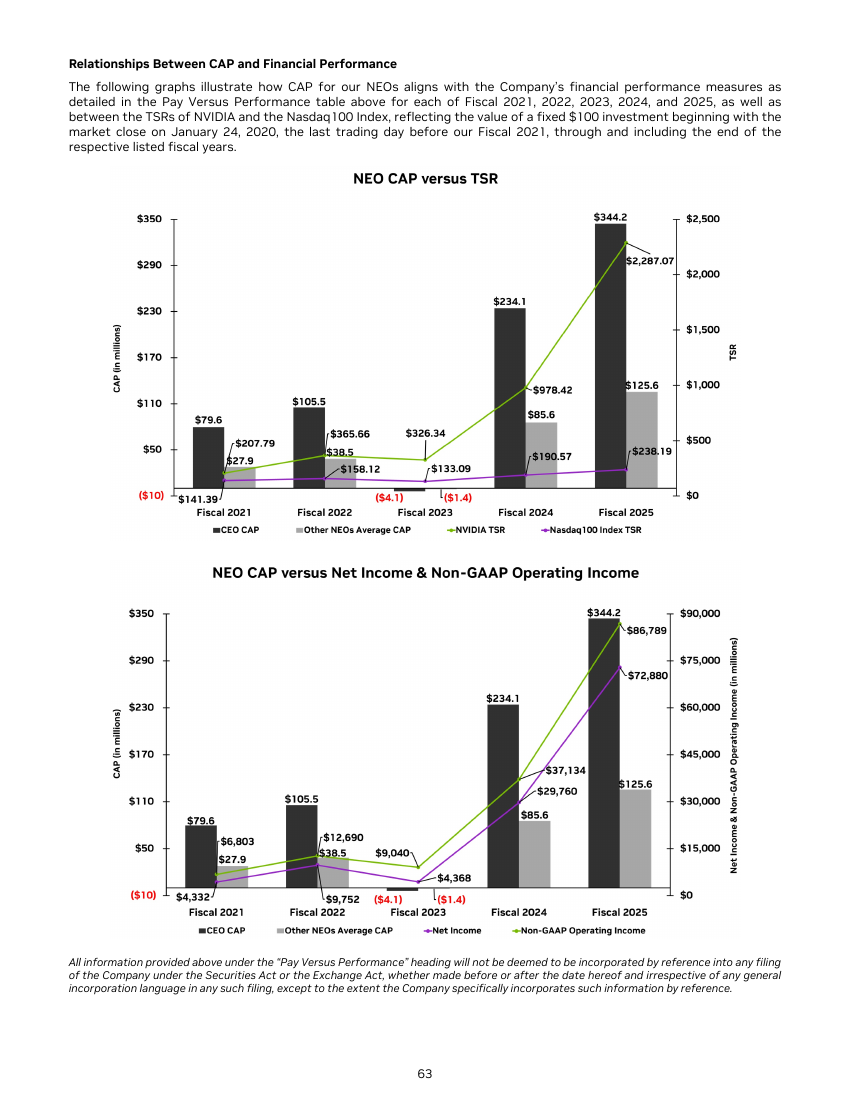
\includegraphics[height=2.4cm]{figs/br1_page76_full.png}};
\node[font=\scriptsize,gray!45!black,below=1pt of pagefull] {page 76 of 181};
\node[inner sep=0,draw=red!60,line width=0.7pt] (cropimg) at (12.9,-4.55)
     {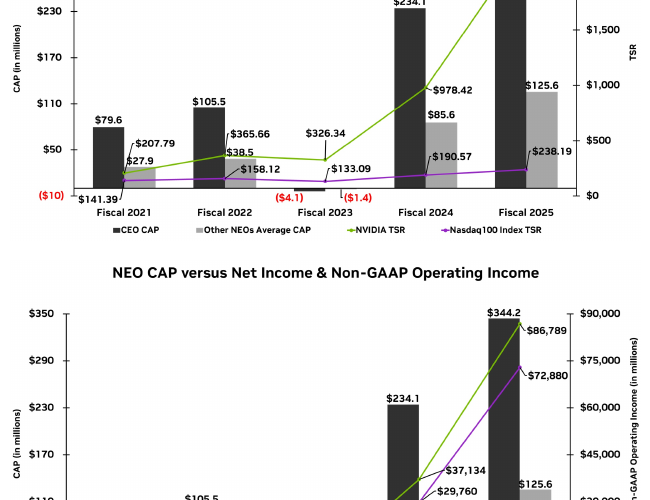
\includegraphics[width=4.7cm]{figs/br1_page76_crop.png}};
\node[font=\scriptsize,red!60!black,text width=5cm,align=center,above=1pt of cropimg]
     {the cropped chart band the agent re-read\\(the Fiscal 2025 bar is clipped off the top)};
\draw[call,-{Latex[length=2mm]}] (pagefull.south) -- node[right,font=\scriptsize,black]{crop \& zoom} (cropimg.north east);
\draw[red!60,dashed,-{Latex[length=2mm]}] (s4.north east) to[out=35,in=180] (cropimg.west);
\end{tikzpicture}%
}
\caption{Active-perception loop on a 181-page business report (NVIDIA annual review), RLM, 16 iterations, \textbf{correct} (gold and predicted 2048.88). Question: \emph{``In Fiscal 2025, by how many dollars does NVIDIA's TSR value exceed the Nasdaq-100 Index TSR value?''} The reasoner surveys the document, locates the table via a table-of-contents pointer, then \textbf{distrusts the full-page read and re-reads a tighter crop} (right) --- which disagrees, exposing a perception error --- adjudicates by reading the region in halves, and does the arithmetic in Python. Every component of the mechanism appears in one trace; the crop-verify catches a wrong number a single read would have submitted.}
\label{fig:trajectory}
\end{figure*}

The same mechanism shows as a head-to-head contrast. On \texttt{science\_poster\_1\_q1} --- ``the percentage score improvement from Baseline to TexTok in rFID-50k for ImageNet 512$\times$512 with 128 tokens'', answer \texttt{30.2\%}, which requires reading two cells (\texttt{1.49}, \texttt{1.04}) from a small table embedded in a 4000$\times$2000 poster and computing $((1.49-1.04)/1.49)\times100$ --- the RLM agent crops the table band, reads each operand with \texttt{batch\_look}, and computes the result in Python, returning \texttt{30.2\%} (correct) in six iterations. ReAct, with no REPL, reads the whole 4000$\times$2000 poster at page granularity, cannot zoom to the cell, terminates in two iterations, and returns \texttt{0.48\%} (wrong). The REPL is the difference between reading a cell and reading a page.

\subsection{Generalization: cross-family and capability-gated}

The advantage is not specific to one model. Two sweeps probe its reach without conflating perception with reasoning: one varies the reasoner while holding perception fixed at the 27B VLM (Table~\ref{tab:scale}), the other compares whole homogeneous models, where the reasoner is also its own VLM, across families (Table~\ref{tab:family}).

\begin{table}[t]
\centering
\small
\begin{tabular}{lccc}
\toprule
Reasoner ($\times$ 27B VLM) & RLM & ReAct & CodeAct \\
\midrule
Qwen3-8B (older gen) & 11.73 & 15.79 & 9.50$^\dag$ \\
Qwen3.5-4B & 21.09 & 15.66 & 22.34 \\
Qwen3.5-9B & 24.54 & 21.01 & 24.26$^\dag$ \\
Qwen3.5-27B & 39.38 & 25.16 & 39.53 \\
\bottomrule
\end{tabular}
\caption{Reasoner scale at fixed perception --- each reasoner paired with the 27B VLM. DocVQA-2026 val, $n{=}8$.}
\label{tab:scale}
\end{table}

With perception held fixed, RLM is at or above ReAct at every Qwen3.5 reasoner size (4B 21.09 vs 15.66, 9B 24.54 vs 21.01, 27B 39.38 vs 25.16), and the corrected CodeAct ties RLM at the two scales where it is complete --- 22.34 vs 21.09 at 4B and 39.53 vs 39.38 at 27B. The older-generation Qwen3-8B is the informative exception: given the same strong 27B perception, it still scores higher under ReAct (15.79) than under RLM (11.73) or CodeAct (9.50). A weak coder cannot drive a code REPL, so handing it one hurts; with perception held constant, the binding constraint here is coding capability.

\begin{table}[t]
\centering
\small
\begin{tabular}{lccc}
\toprule
Model (homogeneous) & RLM & ReAct & CodeAct \\
\midrule
Qwen3.5-4B & 12.49 & 11.94 & 16.25 \\
Qwen3.5-9B & 16.67 & 14.97 & 19.35$^\dag$ \\
Qwen3.5-27B & 39.38 & 25.16 & 39.53 \\
Gemma-4-31B & 32.50 & 18.44 & 29.25$^\dag$ \\
Gemma-4-E4B & 7.34 & 6.09 & 7.66$^\dag$ \\
\bottomrule
\end{tabular}
\caption{Cross-family, homogeneous models --- the reasoner is also its own VLM. DocVQA-2026 val, $n{=}8$.}
\label{tab:family}
\end{table}

Within the Qwen3.5 family the homogeneous ladder rises only with scale: 4B and 9B sit low (RLM 12.49 and 16.67), where reasoner and perception are jointly weak, and only the 27B clears the bar --- and the same 4B nearly doubles, to 21.09, once paired with the strong 27B VLM (Table~\ref{tab:scale}), underscoring the perception bottleneck of \S\ref{sec:mechanism}. The harness ordering then reproduces on a second model family: Gemma-4-31B shows RLM 32.50 $\gg$ ReAct 18.44 (a $+14$pp gap), mirroring Qwen3.5-27B's 39.38 $\gg$ 25.16. The small homogeneous Gemma-4-E4B is the floor control --- all three harnesses land at 6--8, within noise of the $\sim$6.25 official baseline, so at this capacity no scaffold pays off.

Together the sweeps fix the gate as base capability --- reasoning, coding, and vision jointly --- not raw parameter count. A modern Qwen3.5-4B clears it (Table~\ref{tab:scale}); a same-size but weaker Gemma-4-E4B does not (Table~\ref{tab:family}); and an older Qwen3-8B fails even with strong perception, for lack of coding ability (Table~\ref{tab:scale}). The advantage appears once, and only once, the base can drive the loop. ($\dag$~older CodeAct implementation, provisional pending re-run; the 4B and 27B CodeAct cells are the corrected append-only loop, final at $n{=}8$.)
